\documentclass{article}
\usepackage[utf8]{inputenc}
\usepackage[english]{babel}

\usepackage{amsthm}
\usepackage{amsmath}
\usepackage[makeroom]{cancel}
\usepackage{amssymb}
\usepackage{enumitem}

\title{Search for Primes}
\author{Karim El Shenawy}
\date{March 2021}

\usepackage{natbib}
\usepackage{graphicx}

\begin{document}

\maketitle

\section*{Introduction}
This course notebook is the collection of theorem proofs, exercises and answers from Unit 10 of the Number Theory Through Inquiry (Mathematical Association of America Textbooks).

\section*{Theorems from Search for Primes}

\subsection*{10.1 Exercise} 
\quad \textit{If n is a d-digit number, explain why the trial division primality test requires roughly $10^{\frac{d}{2}}$ trials.}

\textit{Solution.} By the trial division primality test a number n is prime if and only if for all primes $p \leq \sqrt{n},$ p does not divide n. The proof is the following

\begin{proof}
Suppose natural number p has no prime divisor less than or equal to $\sqrt{p}$. This implies that p is prime. Now, by contradiction, let's assume that p is composite and each prime divisor $p_i$ of $p$ satisfies $p_i > \sqrt{p}, i \in \mathbf{Z}$. Thus, by the Fundamental Theorem of Arithmetic, $p = p_1p_2...p_k, \exists k \in \mathbf{Z}$. However,
\begin{center}
    $p = p_1p_2...p_k > \sqrt{p}\sqrt{p}p_3...p_k = pp_3...p_k \geq p$.
\end{center}
This shows that $p > p$ which is an obvious contraction. Thus, p must be prime.

Conversely, suppose p is prime. Then the only divisor of p is itself which implies that $p > \sqrt{p}$ since $p  > 1$. Thus, p has no prime divisor less than or equal to $\sqrt{p}$.
\end{proof}

Now back to the question, to test the primality of n, we would need to perform trial divisions by primes that are less or equal to $\sqrt{n}$ if any one of these primes divide n, n is composite. Otherwise, n is prime.\\

Suppose n has d-digits. Then $n < 10^d$. By Prime Number Theorem,
\begin{align*}
    &&\pi(\sqrt{n}) &\approx \frac{\sqrt{n}}{\ln{\sqrt{n}}} &&\\
    &&\pi(\sqrt{n}) &< \frac{c \cdot \sqrt{n}}{\ln{\sqrt{n}}} && (c = \text{ constant})\\
    &&              &< \sqrt{n} && \text{where n is large}\\
    &&      n       &< 10^d && \text{n has d-digits}\\
    &&  \sqrt{n}    &< 10^{\frac{d}{2}} &&
\end{align*}
Therefore, the trial division primality test requires roughly $10^{\frac{d}{2}}$ trials. 

\subsection*{10.2 Exercise} 
\quad \textit{If n is a d-digit number, explain why the Wilson's Theorem primality test requires roughly $10^d$ multiplications.}

\textit{Solution.} By Wilson's Theorem, an natural number n, $n>1$ is a prime if and only if $(n-1)! \equiv -1 \;(\bmod\; n)$. Therefore, to test the primality of a natural number n as a d-digit number, we would have to compute $(n-1)!$ which is $n-1$ number multiplications computed. We know that $n < 10^d$. Thus, the number of multiplications will be roughly $10^d$.

\subsection*{10.3 Question} 
\quad \textit{Suppose that Algorithm A requires $d^2$ steps and Algorithm B requires $2^d$ steps, where d is the number of digits in the number to be tested. Suppose our computer can carry out one million steps per second. How long would it take for our computer to carry out each algorithm when the number to be tested has 200 digits?}

\textit{Solution.}
\begin{itemize}
    \item Algorithm A requires $d^2$. Then $d = 200 \Longrightarrow 200^2 = 40 000$ steps.
    \item Algorithm B requires $2^d$. Then $d = 200 \Longrightarrow 2^200 = 1,6069 \times 10^{60}$ steps.
\end{itemize}
If our computer carries $1 \times 10^6 steps/second$. Then Algorithm A will take less time on our computer.  
\begin{itemize}
    \item Algorithm A takes $\Longrightarrow \frac{40 000}{1 \times 10^6}$ seconds.
    \item Algorithm B takes $\Longrightarrow \frac{1,6069 \times 10^{60}}{1 \times 10^6}$ seconds.
\end{itemize}

\subsection*{10.4 Exercise} 
\quad \textit{Show that the algorithm described in Question 3.6 for computing $a^r \;(\bmod\; n)$ is a polynomial time algorithm in the number of digits in r.}

\textit{Solution.} Let a, n, r and k be natural numbers where k is $0 \leq k \leq n-1$, then we can proceed with the following;
\begin{flalign*}
    && k_1 &\equiv a^2 \;(\bmod\; n)&& \text{$0 \leq k_1 \leq n-1$}\\
    && k_1 \cdot a &\equiv a^3 \;(\bmod\; n)&&\\
    && k_2 &\equiv a^3 \;(\bmod\; n)&& \text{Where $k_2 = k_1 * a$ and $0 \leq k_2 \leq n-1$}\\
    && k_3 &\equiv a^4 \;(\bmod\; n)&& \text{Where $k_3 = k_2 * a$ and $0 \leq k_3 \leq n-1$}\\
    && &... &&\\
    && k_{r} \times a &\equiv a^{r+2} \;(\bmod\; n)&& \text{Where $k_r = k_{r-1} * a$ and $0 \leq k_r \leq n-1$}\\
    && k_{r-1} &\equiv a^{r} \;(\bmod\; n)&&
\end{flalign*}
Thus, you never multiply numbers larger than n. We compute $k_{r} \times a \equiv a^{r+2} \;(\bmod\; n)$ and we recompute the new $k$ with $a$ until $a^r$. Thus, this is a polynomial time algorithm in the number of digits in r.

\subsection*{10.5 Exercise} 
\quad \textit{State the contrapositive of Fermat's Little Theorem.}

\textit{Solution.} The contrapositive of Fermat's Little Theorem is\\
\textit{If there exists a natural number n and some number a for which $a^n - a$ is not divisible by n. Then n is not a prime number.}

\subsection*{10.6 Exercise} 
\quad \textit{Use Fermat's Little Theorem to show that $n = 737$ is composite.}

\textit{Solution.} Let $n = 737$, then we need to find an integer a such that $a^{737}
\equiv$ or $\not\equiv a \;(\bmod\; 737)$. Let's try $a = 2$,
\begin{align*}
    &&\frac{a^{737} - a}{737} &= \frac{2^{737} - 2}{737}&&
\end{align*}
Thus, there is some integer a such that $737 \nmid a^{737} - a$. Therefore, 737 is composite. 

\subsection*{10.7 Question} 
\quad \textit{State the converse to Fermat's Little Theorem. Do you think the converse to Fermat's Little Theorem is true?}

\textit{Solution.} The converse to Fermat's Little Theorem is as follows\\
\textit{If $a^n \equiv a \;(\bmod\; n)$ for all integers a, then n is prime.}\\
The converse part of the Theorem is not true. Let's try an example. with composite number $561 = 3 \cdot 11 \cdot 17$. However, $a^{561} \equiv a \;(\bmod\; 561)$ for all integers a. This is known as the Carmichael Number which is a composite number n such that $b^n \equiv b \;(\bmod\; n)$ for all integers b.

\subsection*{10.8 Theorem} 
\quad \textit{Let n be a natural number greater than 1. Then n is prime if and only if $a^{n-1} \equiv 1 \;(\bmod\; n)$ for all natural numbers a less than n.}

\begin{proof}
Suppose natural number n, $n>1$, is prime. Then by Fermat's Little Theorem $a^{n-1} \equiv 1 \;(\bmod\; n)$ for all integers a, $a<n$.

Conversely, suppose n is not prime. Then by Fundamental Theorem of Arithmetics, $n =p_1p_2...p_k, \exists k \in \mathbf{Z}$ and p is prime. Suppose that $n = n_1 \cdot n_2$ and $n > n_1,n_2$. Thus,
\begin{align*}
    \Longrightarrow\; & n_1^{n-1} &\equiv 1 \;(\bmod\; n)&&\\
    \Longrightarrow\; & n_1^{n-1} - 1 &\equiv 0 \;(\bmod\; n)&&
\end{align*}
Similarly,
\begin{align*}
    \Longrightarrow\; & n_2^{n-1} &\equiv 1 \;(\bmod\; n)&&\\
    \Longrightarrow\; & n_2^{n-1} - 1 &\equiv 0 \;(\bmod\; n)&&
\end{align*}
Then, by $n = n_1 \cdot n_2$,
\begin{align*}
    &&n^{n-1} - 1 &\equiv 0 \;(\bmod\; n)&&\\
    &&(n_1^{n-1} - 1)(n_2^{n-1} - 1) &\equiv 1 \;(\bmod\; n)&&\\
    &&n_1^{n-1}n_2^{n-1} - n_1^{n-1} - n_2^{n-1} + 1 &\equiv 1 \;(\bmod\; n)&&\\
    &&n^{n-1} - n_1^{n-1} - n_2^{n-1} + 1 &\equiv 1 \;(\bmod\; n)&&\\
    &&0 - 1 - 1 + 1 &\equiv 1 \;(\bmod\; n)&&\\
    && - 1 &\equiv 1 \;(\bmod\; n)&&
\end{align*}
Thus, n must be a prime.
\end{proof}

\subsection*{10.9 Question} 
\quad \textit{Does the previous theorem give a polynomial or exponential time primality test?}

\textit{Solution.} The previous theorem must be an polynomial time primality test since we are computing all possible integers a where $a < n$.

\subsection*{10.10 Exercise} 
\quad \textit{Compute $2^{n-1} \;(\bmod\; n)$ for all odd numbers n less than 100. If you have access to a computer, and some computing software, keep going. Test any conjecture you make along the way. State a probably prime test based on your observations.}

\textit{Solution.}\\
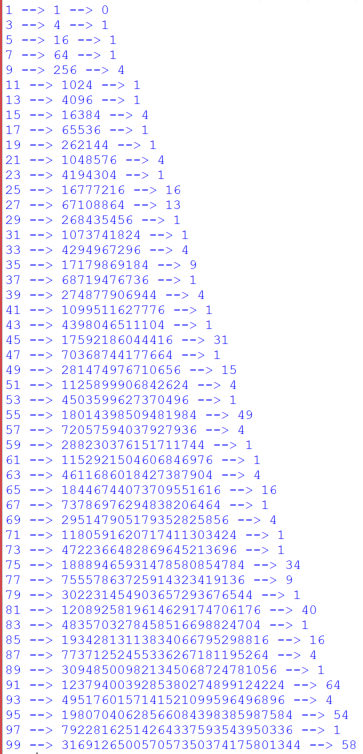
\includegraphics[width=5cm]{odds.PNG}\\
We can observe that all prime odd values n are congruent to 1 modulo n.\\
\textbf{Conjecture.} \textit{For all odd natural numbers n, if $2^{n-1} \equiv 1 \;(\bmod\; n)$ then n is prime.}
\subsection*{10.11 Theorem} 
\quad \textit{Let a and n be relatively prime natural numbers. Then n is prime if and only if $(x+a)^n \equiv x^n+a \;(\bmod\; n)$ for every integer x.}

\begin{proof}
Let a and n be relatively prime natural numbers and n is prime. Suppose $(x+a)^n \equiv x^n+a \;(\bmod\; n)$ for every integer x. By Fermat's Little Theorem, $a^n \equiv a \;(\bmod\; n)$. Then, by direct proof,
\begin{align*}
    &&(x+a)^n &= x^n + nx^{n-1}a + \frac{n(n-1)}{2!}x^{n-2}a^2 + ... + nx^1a^{n-1} + a^n&&\\
    &&(x+a)^n &\equiv (x^n+a^n) \;(\bmod\; n)&&\\
    &&(x+a)^n &\equiv (x^n+a) \;(\bmod\; n)&&
\end{align*}
Conversely, suppose $(x+a)^n \equiv (x^n+a) \;(\bmod\; n)$ then by direct proof,
\begin{align*}
    &&(x+a)^n &= x^n + nx^{n-1}a + \frac{n(n-1)}{2!}x^{n-2}a^2 + ... + nx^1a^{n-1} + a^n&&\\
    &&(x+a)^n &\equiv (x^n+a^n) \;(\bmod\; n)&&\\
    &&(x+a)^n &\equiv (x^n+a) \;(\bmod\; n)&&\\
    &&(x^n+a^n) &\equiv (x^n+a) \;(\bmod\; n)&&\\
    &&a^n &\equiv a \;(\bmod\; n)&&
\end{align*}
Thus, n must be prime, by Fermat's Little Theorem.
\end{proof}

\subsection*{10.12 Blank Paper Exercise} 
\begin{itemize}
    \item Trial division primality test
    \item Wilson's primality test
    \item Fermat's Little Theorem and it's converse
    \item AKS primality test
    \item Pepin's test
    \item Proth's test
    \item Lucas-Lehmer test
\end{itemize}

\section*{Supplementary from Finding Prime Numbers}

\subsection*{10.1.1 Conjecture} 
\quad \textit{Let p be an odd natural number. Then, if any two of the following three conditions hold, so does the third.}
\begin{enumerate}[label=a.]
    \item \textit{$p = 2^k \pm 1$ or $p = 4^k \pm 3$}
    \item \textit{$2^p - 1$ is prime}
    \item \textit{$\frac{2^p+1}{3}$ is prime}
\end{enumerate}

\subsection*{10.1.2 Theorem} 
\quad \textit{If $a_1 \equiv a_2 \;(\bmod\; n)$ then}
\begin{center}
    $(\frac{a_1}{n}) = (\frac{a_2}{n})$.
\end{center}

\begin{proof}
By direct proof,
\begin{align*}
    &&a_1 &\equiv a_2 \;(\bmod\; n) &&\\
    &&a_1 \cdot \frac{1}{n} &\equiv a_2 \cdot \frac{1}{n} \;(\bmod\; n) &&\\
    &&(\frac{a_1}{n}) &\equiv (\frac{a_2}{n}) \;(\bmod\; n) &&
\end{align*}
Then,
\begin{center}
    $(\frac{a_1}{n}) = (\frac{a_2}{n})$.
\end{center}
\end{proof}

\subsection*{10.1.3 Theorem} 
\quad \textit{The Jacobi symbol is multiplicative. That is}
\begin{center}
    $(\frac{a_1a_2}{n}) = (\frac{a_1}{n})(\frac{a_2}{n})$.
\end{center}

\begin{proof}
Suppose that $a_1 \equiv a_2 \;(\bmod\; n)$ then by direct proof,
\begin{align*}
    &&(\frac{a_1a_2}{n}) &= (\frac{a_1}{n})(\frac{a_2}{n}) &&\\
    &&a_2(\frac{a_2}{n}) &= (\frac{a_2}{n})(\frac{a_2}{n}) && \text{By Theorem 10.1.2}\\
    &&a_2 &= (\frac{a_2}{n}) &&
\end{align*}
Now, if $a_2 \;(\bmod\; n)$ is a quadratic residue then $(\frac{a_2}{n}) = 1$. Similarly, if $a_2 \;(\bmod\; n)$ is not a quadratic residue then $(\frac{a_2}{n}) = -1$. Either or, since $n \mid a$, then $(\frac{a_2}{n}) = 0$ which would suggest that $a_2 = 0$ as well.
\end{proof}

\subsection*{10.1.4 Theorem} 
\quad
\begin{equation*}
(\frac{2}{n}) = \left\{
        \begin{array}{ll}
            1 & \quad n = \pm 1 \;(\bmod\; 8)\\
            -1 & \quad n = \pm 3 \;(\bmod\; 8)\\
        \end{array}
    \right.
\end{equation*}

\begin{proof}
Identifying two cases:
\begin{itemize}
    \item Case 1: $n = \pm 1 \;(\bmod\; 8)$ then $2 \;(\bmod\; n)$ is a quadratic residue thus $(\frac{2}{n}) = 1$.
    \item Case 2: $n = \pm 3 \;(\bmod\; 8)$ then $2 \;(\bmod\; n)$ is not a quadratic residue thus $(\frac{2}{n}) = -1$.
\end{itemize}
\end{proof}

\subsection*{10.1.5 Theorem} 
\quad \textit{If a and n are odd, then}
\begin{equation*}
(\frac{a}{n}) = \left\{
        \begin{array}{ll}
            -\frac{n}{a} & \quad a \equiv n \equiv 2 \;(\bmod\; 4)\\
            \frac{n}{a} & \quad \text{otherwise}\\
        \end{array}
    \right.
\end{equation*}

\begin{proof}
Incomplete.
\end{proof}

\subsection*{10.1.6 Exercise} 
\quad \textit{Use Theorems 10.1.2-10.1.5 to compute $\frac{122}{329}$ and $\frac{1240}{3003}$.}

\textit{Solution}
\begin{itemize}
    \item $(\frac{122}{329})$ 
    \begin{align*}
        &&(\frac{122}{329}) &= (\frac{61 \times 2}{329})&&\\
        &&                  &= (\frac{61}{329})(\frac{2}{329})&&\\
        &&                  &= (\frac{24}{61})(1)&&\\
        &&                  &= (\frac{-12}{61})(1)&&\\
        &&                  &= (\frac{6}{61})(1)&&\\
        &&                  &= (\frac{-3}{61})(1)&&\\
        &&                  &= (-\frac{1}{3})(1)&&\\
        &&                  &= -1(1)&&\\
        &&                  &= -1&&\\
    \end{align*}
    \item $(\frac{1240}{3003})$ 
    \begin{align*}
        &&(\frac{1240}{3003}) &= (\frac{620 \times 2}{3003})&&\\
        &&                  &= (\frac{620}{3003})(\frac{2}{3003})&&\\
        &&                  &= (\frac{310}{3003})(\frac{2}{3003})(-1)&&\\
        &&                  &= (\frac{155}{3003})(\frac{2}{3003})(-1)(-1)&&\\
        &&                  &= (\frac{58}{155})(-1)(-1)(-1)(-1)&&\\
        &&                  &= (\frac{29}{155})(\frac{2}{155})&&\\
        &&                  &= (\frac{29}{155})(-1)&&\\
        &&                  &= -(\frac{10}{29})&&\\
        &&                  &= -(\frac{5}{29})(\frac{2}{29})&&\\
        &&                  &= -(\frac{4}{5})(-1)&&\\
        &&                  &= (\frac{2}{5})(\frac{2}{5})(-1)&&\\
        &&                  &= (\frac{1}{5})(\frac{2}{5})&&\\
        &&                  &= (-1)(-1)&&\\
        &&                  &= 1&&\\
    \end{align*}
\end{itemize}

\subsection*{10.1.7 Theorem} 
\quad \textit{Let n be prime. Then}
\begin{center}
    $(\frac{a}{n}) \equiv a^{\frac{n-1}{2}} \;(\bmod\; n)$.
\end{center}

\begin{proof}
Incomplete.
\end{proof}

\subsection*{10.1.8 Exercise} 
\quad \textit{Make use of Theorem 10.1.7 to devise a probabilistic primality test, and state with what probability a number will be certified as prime.}

\textit{Solution.} If n is prime then 
\begin{center}
    $(\frac{a}{n}) \equiv a^{\frac{n-1}{2}} \;(\bmod\; n)$.
\end{center}
Tested on a computer and gotten the result of 91\% correct.

\subsection*{10.1.9 Lemma} 
\quad \textit{Let p be prime and write $p-1 = 2^sm$ where $m \geq 1$ is odd. Then for all numbers a, $1 \leq a \leq p-1$, either $a^m \equiv 1 \;(\bmod\; p)$, or there is an r, $1 \leq r \leq s-1$ such that $a^{2^rm} \equiv -1 \;(\bmod\; p).$}

\subsection*{10.1.10 Exercise} 
\quad \textit{State the contrapositive form of Lemma 10.1.9.}

\textit{Solution.} Suppose that for all numbers a, $1 \leq a \leq p-1$, either $a^m \equiv 1 \;(\bmod\; p)$, or there is an r, $1 \leq r \leq s-1$ such that $a^{2^rm} \equiv -1 \;(\bmod\; p).$ If we can write  $p-1 = 2^sm$ where $m \geq 1$ is odd then p is prime.

\subsection*{10.1.11 Theorem} 
\quad \textit{Let p be an odd natural number and let A be the set of strong liars for p. The number of elements in A is not greater than $\frac{\phi(p)}{4}$.}

\subsection*{10.1.12 Exercise} 
\quad \textit{Devise a probabilistic primality test based on Lemma 10.1.9 and use it to check if 221 is prime, using values of 174 and 137 for a.}

\textit{Solution.} Suppose that 221 is prime. Then by Lemma 10.1.9,
\begin{enumerate}
    \item $p-1 = 220 = 2^sm = 2^2 \cdot 55$ where $m = 55 \geq 1$ and odd
    \item Then, suppose a is 174:
    \begin{align*}
        &&a^m &\equiv 1 \;(\bmod\; p)&&\\
        &&174^{55} &\equiv 1 \;(\bmod\; 221)&&\\
        &&47 &\not\equiv 1 \;(\bmod\; 221)&&
    \end{align*}
    \item Then, suppose a is 137:
    \begin{align*}
        &&a^m &\equiv 1 \;(\bmod\; p)&&\\
        &&137^{55} &\equiv 1 \;(\bmod\; 221)&&\\
        &&188 &\not\equiv 1 \;(\bmod\; 221)&&
    \end{align*}
\end{enumerate}
Thus, 221 is not prime.
\end{document}